% IE500 Data Mining - final paper (project report).
% LaTeX template of the DWS thesis (thesis.tex), as the course requires.
% Do not change document class, margins, fonts, etc.
\documentclass[a4paper,oneside,bibliography=totoc]{scrbook}

% some useful packages (add more as needed)
\usepackage[utf8]{inputenc}
\usepackage{graphicx}
\usepackage{latexsym}
\usepackage{amsmath}
\usepackage{amssymb}
\usepackage{tabularx}
\usepackage{booktabs}
\usepackage{algorithm} % you can modify the algorithm style to your liking
\counterwithin{algorithm}{chapter} % so that algorithms have chapter numbers as well
\usepackage{algorithmic}
\usepackage{csquotes}
\renewcommand{\algorithmiccomment}[1]{\hfill\textit{// #1}}
\usepackage[usenames,dvipsnames]{xcolor}
\usepackage[colorlinks,citecolor=Green]{hyperref} % you may change/remove the colors
\usepackage[bottom]{footmisc} % footnotes below a figure at the bottom of the page
\usepackage{multicol} % contents in two columns, so that title, contents and AI declaration share page 1
\usepackage{listings} % excerpt of the game file, set as code (as in the proposal)
\lstset{basicstyle=\ttfamily\scriptsize, columns=fullflexible, keepspaces=true,
  backgroundcolor=\color{black!6}, frame=single, rulecolor=\color{black!30}, framesep=3pt,
  xleftmargin=4pt, xrightmargin=4pt, aboveskip=0pt, belowskip=0pt,
  moredelim={[is][\color{BrickRed}]{@}{@}}} % @...@ marks the blunder

% chicago citation style
\usepackage{natbib}
\bibliographystyle{chicagoa}
\setcitestyle{authoryear,round,semicolon,aysep={},yysep={,}} \let\cite\citep
\renewcommand{\bibfont}{\small}
\setlength{\bibsep}{0pt}

% Page limit (12 pages, at most 10 of content): chapters run on instead of starting a new page each.
% Class, margins and fonts stay those of the template.
\RedeclareSectionCommand[style=section, beforeskip=-.9\baselineskip, afterskip=.4\baselineskip,
  font=\Large\sffamily\bfseries]{chapter}
\RedeclareSectionCommand[beforeskip=-.7\baselineskip, afterskip=.25\baselineskip]{section}
\setlength{\textfloatsep}{6pt plus 2pt minus 2pt}
\setlength{\floatsep}{6pt plus 2pt minus 2pt}
\setlength{\intextsep}{6pt plus 2pt minus 2pt}
\setlength{\abovecaptionskip}{3pt}
\renewcommand{\topfraction}{.85}\renewcommand{\bottomfraction}{.5}\renewcommand{\textfraction}{.1}
\renewcommand{\floatpagefraction}{.8}

% Markers for what is not final. Search for \tbd, \stale and \staletable before submitting; none may be left.
% \tbd: a number not computed yet. \stale{x}, and \staletable for a whole table: a number of the earlier runs,
% made with the old 20-ply filter and the old test games (then only the training games were balanced). It
% changes with the rerun (cleanup, selections, Stockfish, steps 2 to 5) and must be replaced by its new value.
\newcommand{\tbd}{\textcolor{red}{\textbf{??}}}
\newcommand{\stale}[1]{\textcolor{BurntOrange}{#1}}
\newcommand{\staletable}{\color{BurntOrange}}

% team number, names and title (shared with the proposal and the presentation)
% Team details shown on the first page of the proposal, the final paper and the presentation.
% This is the only place where they have to be edited.
\newcommand{\TeamNumber}{5}
\newcommand{\TeamMembers}{Omar Ahmed Mohamed Taha Radwan, Yeuk Yu Lam,\\ Laith Philipp Sandouk, Arhan Erdogan,\\ Jonas Stammer, Jaden Tan Eden}
\newcommand{\ProjectTitle}{Predicting Blunders in Online Chess}
\newcommand{\ProjectSubtitle}{Can a Blunder in a Lichess Game Be Foreseen Before the Move Is Played?}
\newcommand{\SubmissionDate}{\today}


\begin{document}

% Course limits: at most 12 pages including the title/contents page and the reference page,
% at most 10 pages of content, no appendix. Title, contents and AI declaration share the first page.
\frontmatter
\KOMAoptions{titlepage=false}
\subject{IE500 Data Mining -- Project Report}
\title{\ProjectTitle}
\subtitle{\ProjectSubtitle}
\author{Team \TeamNumber\\[.3em] \TeamMembers}
\date{\SubmissionDate}
\publishers{{\small Submitted to}\\
  Data and Web Science Group\\
  University of Mannheim\\}
\maketitle

% table of contents
\begingroup%
\hypersetup{hidelinks}% disable link color in TOC only
\setuptoc{toc}{leveldown}% heading as a section, so that it stays on the title page
\setcounter{tocdepth}{0}%
\deftocheading{toc}{}% the heading goes above both columns
\begin{multicols}{2}[\section*{\contentsname}]%
\tableofcontents%
\end{multicols}%
\endgroup

% Declare below which AI tools you used in the process of writing your work,
% including text, image, code, and data generation (required by the course).
\begin{center}
  \textbf{Declaration of Used AI Tools} \\[.3em]
  \footnotesize
  \begin{tabularx}{\textwidth}{@{}lXlc@{}}
    \toprule
    Tool & Purpose & Where? & Useful? \\
    \midrule
    % "Useful?" is the team's own judgement.
    Claude Code (Anthropic) & Coding assistant: writing, reviewing and testing code & \texttt{src/}, \texttt{tests/} & ++ \\
    Claude Code (Anthropic) & LaTeX support: layout, tables, figures, bibliography & report, slides & ++ \\
    Claude Code (Anthropic) & First drafts, shortening and rephrasing of our text & throughout & + \\
    \bottomrule
  \end{tabularx}
\end{center}

% okay, start new numbering ... here is where it really starts
\mainmatter

% ======================================================================================================
% Course outline: application area and goals (0.5 pages)
% Checklist: the actual problem in the domain, the target variable, classification or regression.
\chapter{Application Area and Goals}
\label{ch:goals}
\suppressfloats[t] % the report starts with its text, not with a figure or table

Lichess, a free chess server, publishes every rated game played on it, 89,616,462 in September 2026 alone
\cite{lichessdb}. Many of these games are not won by better plans or tactics, but instead by the opponent 
making one bad move. Lichess calls such a move a \emph{blunder}: it lowers the mover's
chance of winning, a logistic function of the Stockfish evaluation \cite{lichessaccuracy}, by at least 15
percentage points \cite{lichessadvice}; analysed games mark it with ``??''.

An engine tells how good a position is under perfect play. It does not tell how likely a human of a given 
proficiency, with a given time left, is to go wrong in it. Earlier work predicted which move a player of a given rating chooses
\cite{mcilroyyoung2020maia}; This project attempts to answer the question: \emph{Can a model predict whether a player will blunder on their next
move, from what is known before it: clocks, position, evaluation, ratings and the course of the game?} Such a
model could show players when they tend to blunder, show viewers how hard a position is for the humans at the
board, and tell when decisions under time pressure fail.

The target is the ``??'' of a move: binary classification of moves, with about \stale{5.5}\,\% blunders. This project has 4 main
goals: (1)~\emph{prediction}: beat the strongest simple baseline, the blunder rate per speed, rating and time
left, in Average Precision and log loss on unseen games; (2)~\emph{explanation}: find which information
carries the signal, in particular what an engine adds, with readable rules; (3)~\emph{robustness} across
speeds, ratings and game phases; (4)~\emph{sample design}: test whether training games balanced to the month's
blunder rates give better models than a stratified random draw. After a profile of the data
(Chapter~\ref{ch:data}), Chapters~\ref{ch:selection} to~\ref{ch:evaluation} follow the five steps of the
knowledge discovery process \cite{fayyad1996kdd}, as does our code (Figure~\ref{fig:process});
Chapter~\ref{ch:results} answers the question.

% figures/process.drawio, exported with draw.io: draw.io -x -f pdf --crop -o process.pdf process.drawio
\begin{figure}[hb]
  \centering
  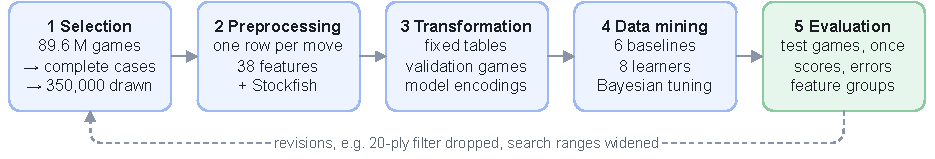
\includegraphics[width=\textwidth]{figures/process}
  \caption{The five steps of the process, one chapter each (Chapters~\ref{ch:selection}--\ref{ch:evaluation}) and
    one folder of our code each. Dashed: results that sent us back to an earlier step.}
  \label{fig:process}
\end{figure}

% ======================================================================================================
% Course outline: profile (structure and size) of the data set, at least 1 page.
% Checklist: distribution of the target, all attributes and their types, data quality, correlation.
\chapter{Data Set Profile}
\label{ch:data}

We use the Lichess Open Database \cite{lichessdb}, licence CC0, one file per month, and take September 2026,
the latest complete month when we started: 89,616,462 games in 29.2~GB of zstd-compressed PGN text; August
2026 serves only to check whether the blunder rate changes between months. A game is a block of 17 header
lines and one line of moves (Figure~\ref{fig:blunder}). Every move carries the mover's clock and, in games a
player had analysed, the Stockfish evaluation after it and the marks \texttt{?!} (inaccuracy), \texttt{?}
(mistake) and \texttt{??} (blunder). Table~\ref{tab:attributes} lists every attribute. The most important are
the ratings (Glicko-2, called Elo in the file), \texttt{TimeControl} (start time and increment, from which
Lichess derives the speed; \citealp{scalachessspeed}), the clock and the evaluation.

% an excerpt of a game of the month, as in the proposal (whose board figure is submission/proposal/blunder_example.pdf)
\begin{figure}[htb]
\begin{lstlisting}
28. cxd5 { [%eval -0.36] [%clk 0:00:40] } 28... cxd5 { [%eval -0.32] [%clk 0:06:22] }
29. @Qc3??@ { [%eval -9.42] [%clk 0:00:18] } 29... Qxc3 { [%eval -9.41] [%clk 0:06:18] } 0-1
\end{lstlisting}
  \caption{Two moves of a game (\href{https://lichess.org/Eh02O2q8}{\texttt{lichess.org/Eh02O2q8}}): with 40
    seconds left against 6:22, White hangs the queen; White's chance of winning falls from 47\,\% to 3\,\%.}
  \label{fig:blunder}
\end{figure}

\begin{table}[tb]
  \centering\footnotesize
  \caption{The attributes of a game: \checkmark{} used for features, F only to filter or draw games, T target,
    $\times$ removed. Counts from the first 42,759 games of the month.}
  \label{tab:attributes}
  % header fields and counts: first three zstd frames of lichess_db_standard_rated_2026-09.pgn.zst
  \begin{tabularx}{\textwidth}{@{}llXc@{}}
    \toprule
    Attribute & Type & Values & Use \\
    \midrule
    \texttt{Event} & categorical & \texttt{Rated Blitz game}, \dots{} \texttt{tournament}, \dots{} \texttt{swiss} & \checkmark \\
    \texttt{Site} & identifier & link to the game, e.g.\ \texttt{lichess.org/mQMQpBqI} & F \\
    \texttt{UTCDate}, \texttt{Date}, \texttt{Round} & date, constant & day of the game; always \texttt{-} & $\times$ \\
    \texttt{UTCTime} & time & start of the game (UTC), e.g.\ \texttt{00:33:03} & \checkmark \\
    \texttt{White}, \texttt{Black} & identifier & user names, about 24,600 distinct ones each & $\times$ \\
    \texttt{White/BlackElo} & integer & rating before the game, e.g.\ \texttt{1500} & \checkmark \\
    \texttt{White/BlackTitle} & categorical & \texttt{BOT}, \texttt{FM}, \dots; in 1\,\% of the games & F \\
    \texttt{TimeControl} & categorical & start time + increment in seconds, e.g.\ \texttt{180+0} & \checkmark \\
    \texttt{ECO}; \texttt{Opening} & categorical & opening code, 395 values; name, 1,672 values & \checkmark; $\times$ \\
    \texttt{Termination} & categorical & \texttt{Normal}, \texttt{Time forfeit}, \texttt{Abandoned}, \dots & F \\
    \texttt{Result}; \texttt{RatingDiff} & categorical; integer & \texttt{1-0}, \dots; rating change through the game & $\times$ \\
    \midrule
    move; \texttt{[\%clk]} & categorical; duration & e.g.\ \texttt{Qc3}; the mover's time left after the move & \checkmark \\
    \texttt{[\%eval]} & numeric & evaluation after the move in pawns, or \texttt{\#n} for mate in $n$ & \checkmark \\
    \texttt{?!}, \texttt{?}; \texttt{??} & categorical & inaccuracy, mistake; blunder (earlier moves: feature) & \checkmark; T \\
    \bottomrule
  \end{tabularx}
\end{table}

\textbf{Quality and target.} The file is written by the server, so ratings and clocks are numbers and moves are
legal, which Chapter~\ref{ch:preprocessing} checks rather than assumes. Clocks are in almost every game, but
evaluations and marks only in analysed ones, about 10\,\% of the month; games without them have no label and
cannot be imputed, so such games are dropped. Of the \stale{580} million moves of the complete games, \stale{5.51}\,\% are
blunders (August: \tbd\,\%; a model learns the rate of its month, a \emph{monthly bias}). Naively predicting no
blunders results in the model being right on \stale{94.5}\,\% of the moves, so accuracy cannot judge our models. The
rate depends on the situation (Figure~\ref{fig:rates}). In a first sample of \stale{945,171} moves it was
\stale{7.8}\,\% below a rating of 1,200 and \stale{3.9}\,\% from 2,000 on, \stale{8.2}\,\% with less than a
twentieth of the time left and \stale{4.8}\,\% with more than half, and \stale{27.7}\,\% right after the
opponent lost 20 points of win probability, against \stale{4.3}\,\% otherwise. The baseline builds on rating and
time left, our features on all three; Chapter~\ref{ch:preprocessing} relates every feature to the target.

\begin{figure}[tb]
  \centering
  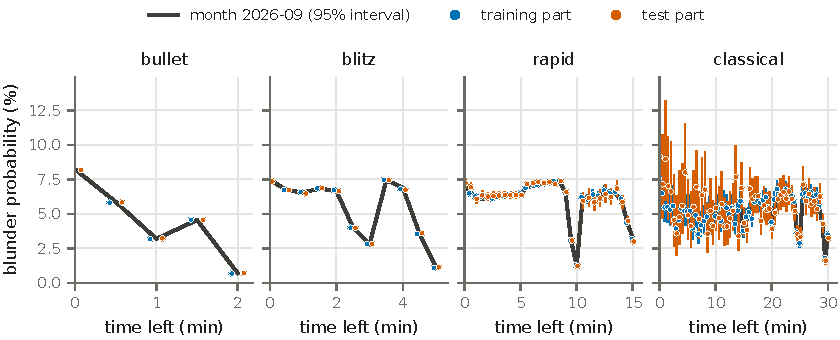
\includegraphics[width=.75\textwidth]{figures/rate_by_time_left}%
  \caption{Blunder rate by time left and speed: the month (line), training and test games (points). Dips at the
    common start times are opening moves played with a full clock. \stale{[earlier run]}}
  \label{fig:rates}
\end{figure}

% ======================================================================================================
% Step 1 of the process (src/01_selection/).
\chapter{Selection}
\label{ch:selection}

The month holds far more games than an engine can analyse in our time, so the first step decides which games are
usable and which of them we draw (Figure~\ref{fig:selection}).

% figures/selection.drawio, exported like figures/process.drawio
\begin{figure}[tb]
  \centering
  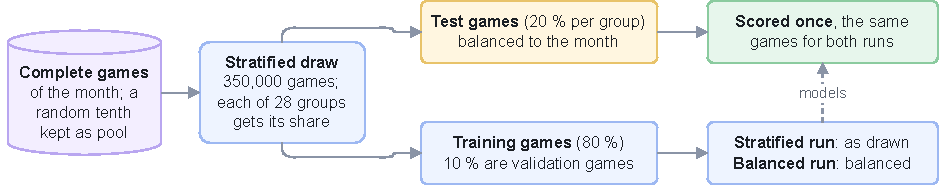
\includegraphics[width=\textwidth]{figures/selection}
  \caption{From the month to the games each part of the work sees; no game is both a test and a training game.}
  \label{fig:selection}
\end{figure}

\textbf{Complete cases.} One pass over the month keeps the complete cases (Table~\ref{tab:funnel}). We used the following filters: (1) 4 speeds from bullet to classical (Lichess's
classes of the estimated duration; \citealp{scalachessspeed}). ultrabullet speed leaves no time to think and
correspondence no time pressure, hence both were excluded; (2) evaluations present, as only analysed games have labels; (3) both ratings known, as
features and strata need them; (4) no computer player, as we model humans; (5) ended normally or on time, as abandoned
games say nothing about decisions; (6) overall moves (at least one move, all legal, each with a clock and an evaluation excluding a mating last move). 
We first also required 20 plies (individual turns) but dropped this filter, as early resignations often
follow early blunders, exactly the moves we want to predict.

\begin{table}[tb]
  \centering\footnotesize
  \caption{Games of September 2026 after each filter step, by speed.}
  \label{tab:funnel}
  % numbers: data/01_selection/september/funnel.csv
  \setlength{\tabcolsep}{4pt}
  \begin{tabular}{@{}lrrrrr@{}}
    \toprule
    Step & bullet & blitz & rapid & classical & all \\
    \midrule
    all games of the file$^a$ & 31,674,536 & 41,228,526 & 15,224,219 & 555,136 & 89,616,462 \\
    bullet to classical, with evaluations & 1,828,324 & 4,000,639 & 2,814,790 & 176,661 & 8,820,414 \\
    ratings, no computer, ended, legal moves & \stale{1,817,714} & \stale{3,957,995} & \stale{2,760,392} & \stale{170,797} & \stale{8,706,898} \\
    clock, evaluation on every move (complete) & \stale{1,817,701} & \stale{3,957,938} & \stale{2,760,358} & \stale{170,792} & \stale{8,706,789} \\
    \midrule
    \multicolumn{6}{@{}l}{\scriptsize $^a$ ``all'' includes 934,045 games of other speeds (ultrabullet,
      correspondence).} \\
    \bottomrule
  \end{tabular}
\end{table}

\textbf{Games, groups and buckets.} Stockfish needs about 40~ms per position, \stale{6,300} core-hours for all
\stale{580} million moves, so we draw 350,000 games, about 250 core-hours. The unit is the whole game, as the
moves of a game share players, clocks and position: no game gives moves to both training and test. Games fall
into 28 \emph{groups}, four speeds times seven bands of the players' mean rating (below 750, steps of 250, 2,000
and above); moves fall into 756 \emph{buckets}, speed $\times$ the mover's rating band $\times$ time left in
30-second steps, the three factors of Chapter~\ref{ch:data} (the time left changes with every move, so it can
only define buckets of moves). The buckets give the baseline and the checks. Every game has fixed random
numbers, hashes of a seed and its id, so every draw from the pool (\stale{871,412} games) can be repeated.

\textbf{Three designs.} A \emph{random} draw gives every group its share of the month only on average. We settled on a
\emph{stratified} draw, as it gives it exactly and draws at random inside each group, removing this chance variation
\cite{cochran1977sampling}. A
\emph{balanced} draw then swaps single games for spare games of the same group, whenever this brings the buckets'
blunder rates as a whole closer to the month's, keeping each bucket's share of moves. The balanced draw sample matches the
month in every combination of speed, rating and time left. However, it chooses games by their label,
replacing games with blunders by calmer ones, which may bend relations we do not watch. Following the
lecturer's advice, we balanced the \emph{test} games so that test scores do not depend on chance deviations of
70,000 games. This can only favour the bucket-rate baseline, which predicts exactly the month's rates, so a
model's lead over it is conservative. Whether balancing the \emph{training} games helps is goal~4, so the
\emph{stratified} and the \emph{balanced run} differ only there.

\textbf{Check.} We sum the buckets' squared deviations from the month's rates, in standard errors, to $\chi^2$
and compare it with 20 fresh stratified draws. The stratified run's training games ($\chi^2 = \stale{1{,}034}$
over \stale{742} buckets) lie within the draws' 5th to 95th percentile (\stale{877--1,095}): as close to the
month as chance allows. Balancing replaced \tbd{} test games and \stale{6.6}\,\% of the training games and
removed almost all deviation ($\chi^2 \approx \stale{30}$). Training and test parts hold \stale{280,002} and
\stale{69,998} games, \stale{18.7} and \stale{4.7} million moves.

% ======================================================================================================
% Step 2 of the process (src/02_preprocessing/). Checklist: missing values, outliers, validity,
% inconsistencies, duplicates, normalisation, feature generation, feature subset selection, external knowledge.
\chapter{Preprocessing}
\label{ch:preprocessing}

The second step turns the games into one row per move with what is known before it (Figure~\ref{fig:cut}),
adds an engine's view, and cleans and reduces the features.

\textbf{Features.} We replay every game with python-chess \cite{pythonchess}. A move in the file holds only a
clock, an evaluation and a mark, so we generated 38 features in six groups: \emph{game}
(speed, start time, increment, colour, move number, hour, kind of event, opening family), \emph{rating} (the
mover's, the opponent's, their difference), \emph{clock} (both clocks; the clock as a share of the estimated
duration, as 30 seconds mean little in classical and much in bullet; their difference; the time spent on recent
moves), \emph{evaluation} (before the move, also as the mover's win probability), \emph{history}, as one error
follows another (the win probability lost by the mover's last, last five, all and worst moves, their errors so
far, the moves since the last one, and the opponent's recent losses and errors), and \emph{board} (legal moves,
check, material of both sides, difference, total).

% figures/known_before.drawio, exported like figures/process.drawio; at the foot of the page, so that it does not
% come before the chapter heading
\begin{figure}[b]
  \centering
  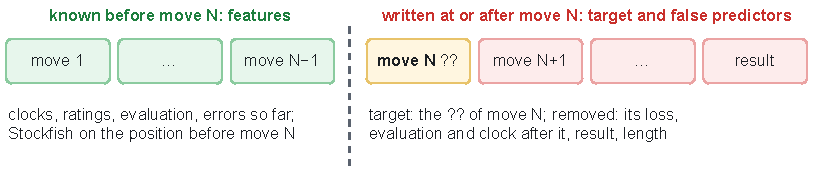
\includegraphics[width=.94\textwidth]{figures/known_before}
  \caption{What the row of move $N$ may know. The leakage check scrambles everything right of a random cut;
    nothing left of it may change.}
  \label{fig:cut}
\end{figure}

\textbf{False predictors and leakage.} The label follows from the evaluation after the move, so a feature that
sees the move or anything later gives the answer away \cite{kaufman2012leakage}. We extract, and then visibly
remove 13 such columns: the move's mark, loss, evaluation, clock and time spent; the game's result, rating
changes, termination and length; the opening's name and its letter before ply~12, which Lichess derives from
later moves; and the player names, which would let a model memorise players instead of situations. The leakage
check cut \stale{2,000} random games (\stale{100} also with Stockfish): no feature left of the cut changed, while
the label of the cut move changed in \stale{673} games, so a feature reading it would have been caught.

\textbf{External knowledge: Stockfish.} The file's evaluation describes the position, not the potential \emph{choices} the
mover faces: where one move holds and thirty lose, a blunder is likely; where almost all are fine, it is not. We
combined it with Stockfish~19 \cite{stockfish} on the position before every move, never looking at the move played. A depth-10 search gives the win probability after the best move and how much the second to fifth best
lose against it. A cheap depth-4 score of every legal move, enough to see a hanging queen, provides 15 columns: the losses of
the five worst moves, the number of moves within an inaccuracy of the best, the shares of moves losing at least
an inaccuracy, a mistake or a blunder, and the number of moves scored. The passes take 31 and 8~ms per position on one core,
against 136~ms for depth 10 on every move; the \stale{24.4} million positions took \stale{15} hours on 16 cores.

\textbf{Cleaning.} \emph{Missing values} are structural (no earlier move before the first); dropping them would
remove all openings, so Chapter~\ref{ch:transformation} fills and marks them. \emph{Outliers}: mate scores have
no pawn value, so evaluations are capped at $\pm$10 pawns, as in Lichess's win probability. \emph{Validity}:
ratings must be numbers and moves legal and timed; the leakage check confirms that each player's first clock
equals the start time.
\emph{Duplicates}: each selected game id must occur exactly once in the pool, or the selection stops.
\emph{Normalisation}: \texttt{Event} names speed and kind of game in several forms (\texttt{Rated Blitz game},
\texttt{Blitz swiss \dots}), which we map to one speed and one kind.

\textbf{Reduction.} Redundant features slow training on 18 million rows, make linear coefficients unstable and split one
signal's importance between copies, so we select features by three fixed rules on 70,000 training games.
\emph{Domain}: we drop features that follow from kept ones (the opponent's rating and clock, both sides'
material, the evaluation in pawns) or that kept ones already cover (start time and increment, carried by
speed and the clock share). \emph{Redundancy}: of two features with Spearman $|\rho| \ge 0.9$, we drop the
less informative. \emph{Weakness}: we drop features whose mutual information with the target, which unlike
$\rho$ also captures non-linear relations, is below 1\,\% of the best feature's. Speed, rating and clock,
on which the buckets rest, are always kept, as are move number and total material despite $\rho \approx
-0.9$, since one measures how far the game has progressed and the other how simplified the position is.
Domain removes \stale{7} features, redundancy none and weakness \stale{5} (colour, hour, kind of event,
rating gap, check), leaving \stale{26}; boosting scored the same without them. With Stockfish only
engine columns may go (\tbd{} of 15 remain), so leaving them out gives exactly the features without the engine. The repository
documents every removal with the measured numbers.

% ======================================================================================================
% Step 3 of the process (src/03_transformation/).
\chapter{Transformation}
\label{ch:transformation}

The third step brings the features into the form each method needs. \textbf{Shared tables} are written once,
with nothing learned from the data: fixed category lists (speed, opening family), so that training and test
games get the same codes; booleans as 0/1; 32-bit floats, which halve the memory of 23 million rows. The
\emph{validation games} (Figure~\ref{fig:selection}), a fixed tenth of the training games chosen by a hash of
their id, choose every setting and stopping point for every method, so the test games are used once. \textbf{What
depends on the data} is fitted inside each model's pipeline on the fitting moves only, so that validation and
test games never influence it and the tuning can choose between encodings. For naive Bayes, logistic regression,
SVM and network, a gap is filled with the median and marked by an indicator, so that ``no earlier move yet''
stays visible; numbers are standardised (for naive Bayes optionally mapped to a normal distribution) and
categories one-hot encoded. Trees take categories as codes and route gaps themselves. \textbf{No binning, no
resampling.} Trees find their own thresholds, and the baseline's buckets already are a binning. Resampling the
classes would shift every probability, while the applications need a risk, log loss rewards a correct one, and
Average Precision depends only on the order; a cut-off for yes or no is chosen afterwards.

% ======================================================================================================
% Step 4 of the process (src/04_data_mining/). Course outline: approaches and parameter settings tried.
% Checklist: baselines, at least one symbolic and one non-symbolic approach, hyperparameter tuning.
\chapter{Data Mining}
\label{ch:mining}

Every method gives a blunder probability per move and is fitted on the training games without the validation
games, every learner both on the \emph{context} features and on \emph{engine} (context plus Stockfish), to show
what the engine adds. Table~\ref{tab:methods} lists the learners; all but XGBoost
\cite{chen2016xgboost} are from scikit-learn \cite{pedregosa2011sklearn}.

\begin{table}[b] % at the foot of the page, so that it does not come before the chapter heading
  \centering\footnotesize
  \caption{The learners with their trials and the search ranges of their hyperparameters (lr: learning rate; log
    scale where marked; first-round limits in brackets). The chosen values are in each run's \texttt{run.json}.}
  \label{tab:methods}
  \begin{tabularx}{\textwidth}{@{}lX@{}}
    \toprule
    Learner (trials) & Hyperparameters and ranges \\
    \midrule
    Naive Bayes (25) & quantile or standard scaling; variance smoothing $10^{-4}$--10 [1] (log) \\
    Logistic regression (10) & $C$: $10^{-3}$--$10^{2}$ (log) \\
    Linear SVM (20) & L2 penalty $\alpha$: $10^{-8}$--$10^{-1}$ [$10^{-2}$] (log); up to 50 [20] epochs \\
    Decision tree (20) & depth 2--24 [16]; moves per leaf 100--10,000 (log) \\
    Random forest (16) & moves per leaf 5 [20]--2,000 (log); features per split $\sqrt{p}$, $0.3p$, $0.5p$ \\
    Gradient boosting (25) & lr 0.02--0.3, leaves 15--255, leaf size 20--5,000, L2 $10^{-3}$--30 (all log) \\
    XGBoost (30) & lr 0.02--0.3, child weight 1--1,000, L2 $10^{-3}$--30 (log); depth 3--10; row and column
      share 0.5--1, 0.4--1 \\
    Neural network (20) & layers (32), (64, 32), (128, 64), (256, 128) [not 256]; L2 $10^{-6}$--$10^{-1}$
      [$10^{-2}$], lr $3\cdot10^{-4}$--$10^{-2}$ [$3\cdot10^{-3}$] (log); up to 100 [50] epochs \\
    \bottomrule
  \end{tabularx}
\end{table}

\textbf{Baselines.} The \emph{bucket rate} predicts the month's blunder rate of the move's bucket, pulled towards
its speed-and-rating rate by 50 moves so that thin buckets get no extreme rates. It is the strongest rule without
learning: a model that does not beat it has learned nothing beyond speed, rating and time pressure. Five simpler
rules show what single variables give: the overall rate (majority class as a probability) and the
rate per speed, per speed and rating, per band of the win probability, and after an opponent's mistake.

\textbf{Learners.} \emph{Naive Bayes} assumes independent features; ours are correlated, so we expect a fair
order but overconfident probabilities \cite{niculescu2005calibration}. \emph{Logistic regression} is calibrated
and readable but cannot combine features, so a clear lead of the trees means that situations carry more risk
than their parts. The \emph{linear SVM} \cite{cortes1995svm} maximises a margin instead; it is trained by
stochastic gradient descent with class weights (without them it predicts ``no blunder'' everywhere), and Platt
scaling \cite{platt1999} on 20\,\% of the fitting games turns its scores into probabilities. The \emph{decision
tree} \cite{breiman1984cart} is our symbolic method: time pressure sets in below a threshold, which a split
captures together with its interaction with rating; leaf rates are pulled towards the overall rate by 50 moves,
so that no leaf predicts~0. The \emph{random forest} \cite{breiman2001forests} averages 200 deep trees and
lowers variance, \emph{gradient boosting} \cite{friedman2001boosting} adds shallow trees fitted to the remaining
errors and lowers bias; comparing them shows which error limits us. As boosting is expected to be best on tabular
data, we use two implementations, scikit-learn's histogram variant \cite{ke2017lightgbm} and XGBoost. The
\emph{neural network}, a multi-layer perceptron trained with Adam \cite{kingma2015adam}, is our non-symbolic
method; its smooth functions show whether the step-like trees miss gradual effects. $k$ nearest neighbours and
kernel SVMs are too slow for millions of rows.

\textbf{Tuning.} Every learner is tuned by Bayesian optimisation with the tree-structured Parzen estimator
\cite{bergstra2011tpe} of Optuna \cite{akiba2019optuna}, which, unlike a grid, spends its trials where earlier
ones scored well, minimising the validation log loss. A trial fits on whole games with about one million moves,
so that 10 to 30 trials per learner fit into hours; the best settings are refitted on all \stale{16.8} million
fitting moves (five million for forest, network and SVM, for memory). Boosting rounds and epochs stop early on
the loss of the validation games, not of random moves, which would split games. In a first
round five learners chose a value at the edge of its range; as the best value might lie beyond, we widened these
ranges and searched again: the new best values lay inside the old ranges and the test PR-AUC moved by at most
0.004, the width of its intervals. The balanced run reuses these settings, so that only its training games differ.

\textbf{One hold-out instead of cross-validation.} With \stale{1.9} million validation moves a trial's score
barely depends on which games are held out, while the 5-fold cross-validation of our proposal would cost five
times as much. We checked this: on five folds of the tuning games, the best setting beat the second best in
\stale{four or five} folds wherever the two differed clearly, and otherwise they differed by less than
\stale{0.00002} in log loss, a fiftieth of the spread between folds.

% ======================================================================================================
% Step 5 of the process (src/05_evaluation/). Course outline: evaluation setup, analysis of the errors of the
% best method, discussion, comparison to the state of the art (together at least 2 pages).
% Checklist: stratified? cost matrix? tuned ranges? symbolic model analysed? feature impact?
\chapter{Evaluation}
\label{ch:evaluation}

\section{Evaluation Protocol and Metric Rationale}
\label{sec:setupeval}

We evaluate strictly at the game level across 28 strata: 280,000 training games (28,284 validation
games, or 1,863,275 moves, in \emph{stratified}) and 70,000 shared test games of 4,625,657 moves (5.51\,\%
blunders) matched to September~2026 priors via 9,153 swaps ($\chi^2 = 49.2$, mean deviation 0.005\,pp). An
unaltered random test draw verifies split stability in Section~\ref{sec:results}.

Raw accuracies cannot be a metric because 94.5\,\% of the moves are non-blunders; therefore, predicting no
blunders would easily achieve 94.5\,\% accuracy and has zero recall and $F_1$. Accuracies below are
reported solely to document this paradox, and we instead tune PR-AUC \cite{saito2015prc}, log loss, Brier
Skill Score (BSS) vs.\ \texttt{bucket\_rate}, and 20-bin ECE \cite{guo2017calibration}. Downstream
trade-offs use validation cut-offs ($F_1$, $F_{0.5}$, top-$K\%$ budgets) and MCC with 1,000-game bootstrap
intervals.

\section{Model Comparison and Operating Policies}
\label{sec:results}

% NOTE: Local full-data untuned runs on the 2026-11-25 S3 tables are populated for completed methods.
% Replace all rows uniformly from run_models.sh once cluster Optuna tuning + RF/SVM/MLP finish.
\begin{table}[t!]
  \centering\scriptsize\setlength{\tabcolsep}{3.2pt}
  \caption{Test scores on 4,625,657 moves without (\emph{context}) and with (\emph{engine}) Stockfish
    features (\emph{bal.}: balanced training; orange: pending cluster Optuna runs).}
  \label{tab:results}
  \begin{tabular}{@{}lrrrrrrrr@{}}
    \toprule
     & \multicolumn{3}{c}{PR-AUC} & \multicolumn{2}{c}{Log loss} & ROC-AUC & F1 & Lift 5\,\% \\
    \cmidrule(lr){2-4}\cmidrule(lr){5-6}
    Method & context & engine & bal. & context & engine & engine & engine & engine \\
    \midrule
    Bucket rate (month) & \multicolumn{2}{c}{0.083} & 0.083 & \multicolumn{2}{c}{0.2063} & 0.637 & 0.140 & 1.84 \\
    Opponent erred (best rule) & \multicolumn{2}{c}{0.107} & & \multicolumn{2}{c}{0.1983} & 0.643 & 0.255 & 3.49 \\
    Naive Bayes & 0.159 & 0.197 & 0.198 & \stale{0.1949} & \stale{0.1847} & 0.801 & 0.272 & 4.68 \\
    Logistic regression & 0.197 & 0.235 & 0.235 & 0.1836 & 0.1725 & 0.830 & 0.312 & 5.51 \\
    \stale{Linear SVM} & \stale{0.196} & \stale{0.233} & \stale{0.232} & \stale{0.1848} & \stale{0.1720} & \stale{0.832} & \stale{0.310} & \stale{5.47} \\
    Decision tree (depth 8) & 0.217 & 0.242 & \tbd & 0.1755 & 0.1686 & 0.840 & 0.318 & 5.66 \\
    \stale{Random forest} & \stale{0.250} & \stale{0.289} & \stale{0.289} & \stale{0.1688} & \stale{0.1599} & \stale{0.866} & \stale{0.355} & \stale{6.35} \\
    Gradient boosting & 0.265 & 0.311 & 0.311 & 0.1657 & 0.1563 & 0.875 & 0.369 & 6.65 \\
    XGBoost & \textbf{0.266} & \textbf{0.312} & \textbf{0.312} & \textbf{0.1656} & \textbf{0.1560} & \textbf{0.876} & \textbf{0.371} & \textbf{6.67} \\
    \stale{Neural network} & \stale{0.246} & \stale{0.291} & \stale{0.289} & \stale{0.1691} & \stale{0.1594} & \stale{0.868} & \stale{0.357} & \stale{6.38} \\
    \bottomrule
  \end{tabular}
\end{table}

Boosted trees with Stockfish features lead on every metric (Table~\ref{tab:results},
Figure~\ref{fig:roc_pr}): \texttt{xgboost/engine} reaches PR-AUC 0.312 (95\,\% CI $[0.309, 0.314]$) and log
loss 0.1560 vs.\ 0.2063 for \texttt{bucket\_rate/month} (BSS $= 0.151$, ECE $= 0.0008$), followed by
histogram gradient boosting (0.311 PR-AUC, 0.1563 log loss, ECE $= 0.0006$). These two ensembles nearly
quadruple the bucket prior (0.083), and flagging opponent errors alone (0.107, lift 3.49$\times$) beats
static lookup. The Stockfish features improve PR-AUC consistently (+0.046 XGBoost, +0.038 logistic
regression), which is an important tactical signal to the models.

\begin{figure}[t!]
  \centering
  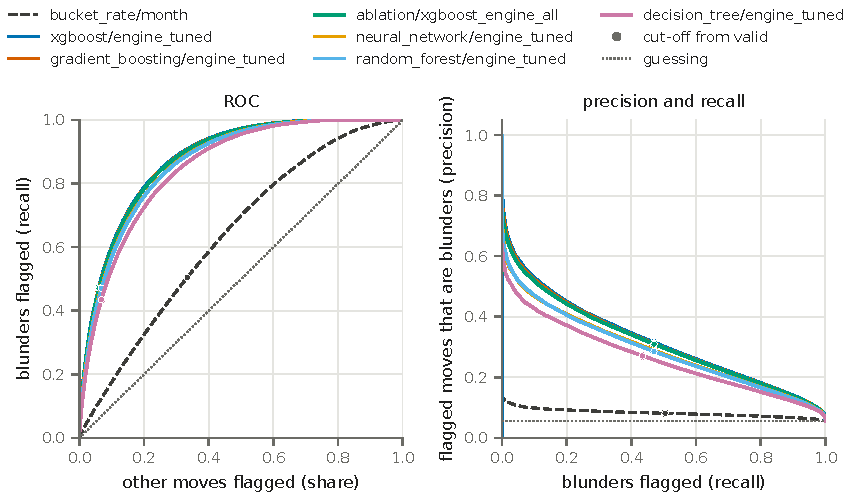
\includegraphics[width=.56\textwidth]{figures/roc_pr}
  \caption{Test ROC (left) and precision--recall (right) curves over 4,625,657 moves.}
  \label{fig:roc_pr}
\end{figure}

Chess board dynamics and structure are reflected by the model gaps, where logistic regression is well
calibrated (ECE $= 0.0020$) but peaked at 0.235 PR-AUC without interactions, and Gaussian Naive Bayes
(0.197 PR-AUC) is overconfident under correlated features \cite{niculescu2005calibration} (untuned log loss
1.6506, ECE 0.3124; Optuna-smoothed ECE \stale{0.024}). Boosted trees model interactions and missingness
natively, outperforming prior tuned
random forests (\stale{0.289}) and neural nets (\stale{0.291}). Under validation cut-offs for
\texttt{xgboost/engine}, Max-$F_1$ (0.1868) flags 8.2\,\% of moves to catch 46.1\,\% of blunders at 31.1\,\%
precision, cutting accuracy from 94.5\,\% to 91.4\,\% while lifting MCC from 0.000 to 0.334. Conversely,
Max-$F_{0.5}$ (0.2906) alerts on 3.8\,\% at 39.8\,\% precision (7.22$\times$ lift) and the top 1\,\% reaches
51.9\,\% precision (9.41$\times$ lift). Stratified and balanced training match closely (Goal~4: XGBoost
0.3118 vs.\ 0.3122), and scoring all six \emph{context} learners on 69,861 unseen random-draw games
(4,615,279 moves, 5.509\,\% rate) preserves exact rank order ($|\Delta\text{PR-AUC}| \le 0.0018$,
$|\Delta\text{log loss}| \le 0.0003$).

\section{Feature Attribution and Symbolic Rules}
\label{sec:importance}

\begin{table}[t!]
  \centering\scriptsize\setlength{\tabcolsep}{4pt}
  \caption{Feature-group ablation (XGBoost on 5M moves) and permutation log-loss share, pending rerun on the
    33 surviving columns.}
  \label{tab:ablation}
  \staletable
  \begin{tabular}{@{}lrrrrr@{}}
    \toprule
     & \multicolumn{2}{c}{Without the group} & \multicolumn{2}{c}{Only the group} & Shuffled \\
    \cmidrule(lr){2-3}\cmidrule(lr){4-5}
    Group & PR-AUC & Log loss & PR-AUC & Log loss & share \\
    \midrule
    All features & 0.315 & 0.1554 & & & \\
    Engine (7 kept) & 0.263 & 0.1658 & 0.206 & 0.1749 & 48\,\% \\
    History (12 kept) & 0.279 & 0.1602 & 0.219 & 0.1766 & 9\,\% \\
    Evaluation (1 kept) & 0.299 & 0.1587 & 0.104 & 0.1985 & 34\,\% \\
    Board (3 kept) & 0.302 & 0.1576 & 0.105 & 0.1980 & 4\,\% \\
    Rating (1 kept) & 0.308 & 0.1571 & 0.070 & 0.2115 & 2\,\% \\
    Game (3 kept) & 0.313 & 0.1557 & 0.078 & 0.2041 & 2\,\% \\
    Clock (6 kept) & 0.313 & 0.1556 & 0.089 & 0.2022 & 1\,\% \\
    \bottomrule
  \end{tabular}
\end{table}

Stockfish features contribute the most to predictive performance. Removing them causes the largest drop in
Table~\ref{tab:ablation} (PR-AUC 0.315 to 0.263), followed by history (0.279), whereas clock, rating, and
game context contribute little marginal signal once tactical sharpness and prior errors are known. The depth-4
CART tree (16 leaves, PR-AUC 0.198, log loss 0.1764) omits clock and rating entirely and its root tests
\texttt{opp\_last\_loss} $> 0.19$, peaking at
35.45\,\% blunders across 381,295 training moves (6.4$\times$ baseline) with \texttt{opp\_blunders} $> 0.50$,
\texttt{sf\_gap\_5} $> 0.17$, and \texttt{sf\_gap\_2} $> 0.10$, while falling to 0.32\,\% across 3,174,411
quiet moves (\texttt{sf\_share\_blunder} $\le 0.60$, clean 5-move history, worst loss $\le 4$\,pp; 0.00\,\%
when \texttt{eval\_wp} $\le 0.07$).

\section{Error Analysis, Subgroups, and Prior Work}
\label{sec:errors}

\begin{figure}[t!]
  \centering
  \includegraphics[width=.65\textwidth]{figures/error_profile}
  \caption{Error profile of \texttt{xgboost/engine} at Max-$F_1$ (0.1868): subgroup recall (left) and
    row-standardised mean features by confusion cell (right).}
  \label{fig:errors}
\end{figure}

At Max-$F_1$, \texttt{xgboost/engine} flags 377,878 moves (8.2\,\%): 117,364 caught blunders, 137,461 misses,
260,514 false alarms, and 4,110,318 quiet moves (Figure~\ref{fig:errors}). Misses happen in calm states—earlier
moves (22.1 vs.\ 24.2), higher clocks (57.1\,\% vs.\ 51.3\,\%), equal evaluations (0.551 vs.\ 0.640), higher
Elo (1,594 vs.\ 1,466), and sound opponent play (\texttt{opp\_last\_loss} 0.052 vs.\ 0.222)—explaining lowest
recall in openings (36.1\,\%) and 2000+ games (36.1\,\%). False alarms resemble caught blunders pre-move
(\texttt{opp\_last\_loss} 0.191, \texttt{legal\_moves} 32.9) where the mover finds the defence. Across all 26
subgroups (Goal~3), \texttt{xgboost/engine} cuts log loss by 16.3\,\% to 56.0\,\% vs.\
\texttt{bucket\_rate/month} (PR-AUC 0.266--0.457 vs.\ 0.017--0.153).

These findings confirm \citet{anderson2017error}—position difficulty dominates skill and time on modern
Lichess play—while adding recent move history, especially immediately preceding opponent blunders, as a dynamic
signal omitted in cross-sectional models. Unlike move-matching networks such as Maia and Maia-2
\cite{mcilroyyoung2020maia,tang2024maia2}, calibrated risk prediction under PR-AUC makes the empirical
bucket rate our direct benchmark.

% ======================================================================================================
% Checklist: result critically evaluated, compared with the baselines, what it means for the problem.
\chapter{Results}
\label{ch:results}

Yes, a blunder can be foreseen in part before the move is played. On \stale{69,998} unseen games, XGBoost with
our engine features reaches a PR-AUC of \stale{0.321} against \stale{0.082} for the blunder rate per speed, rating
and time left, with a log loss a quarter lower (goal~1). The signal lies in the position and the course of the
game, not in the clock: how many moves lose is the strongest group of features, the last moves of both players the
second, and the readable tree says the same in rules (goal~2). The lead holds in every speed, rating band, game
phase and band of time left (goal~3). Balancing the training games changed no model (goal~4).

\textbf{Limitations.} Only analysed games have labels, and players do not choose at random which games to
analyse, so our rates may differ from those of all games. The labels come from Lichess's server analysis, our
engine features from a shallower search. One month cannot show changes over time, and the same players occur in
training and test games, so a model may partly learn their habits; a split by player would test this.

\textbf{Use.} A lift of \stale{6.8} ranks the dangerous moments of a game well enough for a broadcast or a
training tool (Chapter~\ref{ch:goals}), such as the move after the opponent's mistake. It is no reliable warning
before every blunder: at its cut-off the model catches \stale{47}\,\% of them, and two of three flagged moves are
fine.

\bibliography{references}

\end{document}
